\section{Work Undertaken}
\label{Research}

% In the past year I’ve largely hit the goals agreed upon at the
% last annual review, an overview of which I present here.

\subsection{Mungo}
\label{sub:Mungo}


Mungo\cite{kouzapas16} is a Java front-end tool, developed at the University of Glasgow, used to statically typecheck Java programs augmented with typestate
\Mungo implements two main components. First, a Java-like syntax to define
typestate specifications for classes, and second, a typechecker
that checks whether objects that have typestate specifications are used correctly.

% A protocol or session type is represented as a separate typestate file, associated with a Java class. The protocol definition is described as a sequence of method calls, the order of which determines the validity of the protocol.
%
Typestates are specified in separate files and
are associated with Java classes by means of a Java
annotation. This allows programs that have been
checked by \Mungo to be compiled and run using standard
Java tools.
%
% The declaration of a typestate specification in a single file
% contrasts with other approaches that take the viewpoint
% of typestate as pre- and post-conditions on methods.
% %
%\Mungo allows the programmer to use Java annotations
%to associate a typestate specification file with a Java
%class.
If a class has a typestate specification, the \Mungo typechecker analyses
each object of that class in the program and extracts the
method call behaviour (sequences of method calls) through the object's life. Finally, it checks the extracted information against
the sequences of method calls allowed by the typestate specification.



\Mungo supports typechecking for a subset of Java.
The programmer can define both classes that follow
a typestate specification and classes that do not.
The typechecking procedure follows objects (instances
of the former classes) through argument passing and
return values. Moreover, the typechecking procedure
for the fields of a class follows the typestate
specification of the class to infer a typestate
usage for the fields. For this reason fields that
follow a typestate specification are only allowed to be defined
in a class that also follows a typestate specification.

\Mungo uses the JastAdd framework\footnote{http://jastadd.org/web/extendj/}\cite{jastadd}. The JastAdd framework provides a Java parser
which was used for the implementation of the \Mungo typechecker. The JastAdd suite was also used to implement a parser
for the Java-like typestate specification language.

The following work has been undertaken on the Mungo tool:
\begin{itemize}
  \item The tool has been moved from the Java 1.4 compiler to the Java 1.8 compiler and adapted to work with the new framework.(joint work with Dr. Dimitrios Kouzapas)
  \item Moving the tool to a new compiler framework was a good opportunity for some Refactoring(such as getting rid of dead code or method extraction).
  \item the tool has been extended to support Java enumerations.(joint work with Dr. Dimitrios Kouzapas)
  \item Syntactic support  for annotations
  \item Syntactic support for generic types
  \item Special annotation for typestate
\end{itemize}

Areas of ongoing work:
\begin{itemize}
  \item Update repositories.
  \item Typecheck exceptions.
  Exceptions are supported syntactically but are type-checked under
  the (unsound) assumption that no exceptions are thrown;
  a \lstinline|try{...} catch(Exception e) {...}| statement is typechecked by
  typechecking the try body and if an exception is thrown a typestate violation may result.
  \item Typecheck generic types.
  Generics are currently supported syntactically, but not typechecked.
  \item Extended support for more straightforward Java features such as synchronised statements,
  inner and anonymous classes, or static initialisers.
\end{itemize}

Areas of future work:
\begin{itemize}
  \item typecheck collections
  \item context-free typestates
  \item aliasing
\end{itemize}

\subsection{StMungo}
\label{sub:StMungo}

StMungo (Scribble to \Mungo) \cite{kouzapas16} is a Java-based tool, developed at the University of Glasgow, that translates a Scribble\cite{scribble, YHNN2013} local protocol into a \Mungo specification and skeleton socket-based implementation code. The resulting code is typechecked using \Mungo. Scribble is a protocol description language that can describe how two or more participating entities interact should interact with each other.

After the Scribble protocol is translated to a \Mungo specification, \Mungo\ref{Mungo} is used to generate a Java implementation for the protocol. This tool allows an easy transition from a Scribble global protocol definition to working Java implementation. We start by specifying distributed multiparty protocol in Scribble. We can then use the Scribble toolchain to validate and project the global protocol into a local one describing the interactions from the point of view of a specific participant. For every Scribble local protocol, StMungo will produce .mungo files containing: a typestate specification describing the local protocol as a sequence of method calls, an API for the participant implementing the typestate methods and a main class skeleton calling the methods in the typestate.

To improve this tool various extensions have been implemented:

\begin{itemize}
  \item extended the tool to translate messages with no payload i.e.
  \begin{lstlisting}[basicstyle=\footnotesize]
    message_operator ()
  \end{lstlisting}
  \item extended the tool to translate messages with multiple payload i.e.
  \begin{lstlisting}[basicstyle=\footnotesize]
    message_operator ( payload_type1, ..., payload_typen )
  \end{lstlisting}
  \item extended the tool to translate messages without a message signature i.e.
  \begin{lstlisting}[basicstyle=\footnotesize]
    ( payload_type1, ..., payload_typen )
  \end{lstlisting}
  \item extended the tool to translate messages with annotated payloads i.e.
  \begin{lstlisting}[basicstyle=\footnotesize]
    message_operator ( annotation:payload_type)
  \end{lstlisting}
  \item various small improvements to allow most translations to run without having to be edited by a human
  \item various improvements allowing the tool to crash gracefully
  \item adapted the tool to work with multiple versions of scribble specification
  \item improved the tool by implementing support for special cases of recursions nested in choice structures
  A simple example of a problematic scribble specification is:
  \begin{lstlisting}[basicstyle=\footnotesize]
    global protocol Example(role S, role C) {
    choice at C{
            rcpt(String) from C to S;
        } or {
            msg(String) from C to S;
            rec loop {
                    subject(String) from C to S;
                    continue loop;
                }
            }
        }
    }
  \end{lstlisting}
  \item improved the tool by implementing support for special cases of nested choice inside a recursion

  A simple example of a problematic scribble specification is:
  \begin{lstlisting}[basicstyle=\footnotesize]
  global protocol ProtocolName(role S, role C) {
    command(String) from C to S;
    rec overall {
    choice at S
    	{
    	ok(String) from S to C;
    			choice at S {end(String) from S to C;}
    			or {
    			sum(String) from S to C;
    			}
    			message(String) from S to C;
    	} or {	 error(String) from S to C;	}
    	continue overall;
    }
    }
  \end{lstlisting}
  \item refactoring(such as method extraction or getting rid of dead code) to keep everything simple
  \item regression testing to find any new bugs introduced
  \item collaborated with fellow PhD student Florian Weber on a plug-in for mapping between concrete and abstract messages from Scribble to the `real-world' representation. Author's contributions being: debugging, refactoring, integrating with StMungo, and partly writing a paper(rejected).
\end{itemize}

Areas of further work:
\begin{itemize}
  \item extending the tool to translate to support inlined protocols and sub-protocols(ongoing)
  \item extension to translate more complex constructs such as interruptible or parallel
  \item keeping it up to date with changes in Scribble and \Mungo(ongoing)
\end{itemize}

\subsection{Session type evaluation}

\subsubsection{Usecases}
\label{sub:usecases}

To better understand the expressive power of current session type technology together with any limitations that may need to be addressed, the current use case repository\footnote{https://github.com/epsrc-abcd/session-types-use-cases} was surveyed as a first step. As a second step, new real-world examples were sought. From the various protocols looked after, representations were attempted for two, Paxos and the File Transfer Protocol(FTP).

One protocol chosen was the File Transfer Protocol described by Request for Comments(RFC): 959\cite{FTP-rfc}. FTP is a standard network protocol for transferring  files between a client and server on a network.  FTP is an unusual protocol in that it utilizes two ports, a data port and a command(control) port. FTP may run in active or passive mode, which determines how the data connection is established. In both cases, the client creates a TCP control connection from a random, usually an unprivileged, port number to the FTP server command port 21.

Some representations of the algorithm have been attempted using Scribble, combined with StMungo and Mungo to give a working Java code. However in trying to represent it some shortcomings of StMungo became apparent. Hence, work on an FTP representation has been paused to improve StMungo and Mungo, to allow a better representation. Work on this usecase is planned to be restarted in the autumn.


Another protocol chosen as a usecase was Paxos. Paxos is a protocol for solving consensus in a network of unreliable processes. It ensures that a single value among the proposed values can be chosen. It assumes an asynchronous, non-Byzantine model.\cite{lamport1998part}

Two major advantages of Paxos are that it is provably correct in asynchronous networks that eventually become synchronous and it does not block if a majority of participants are available. Furthermore it has provably minimal message delays in the best case. Despite it's reputation of being difficult to understand \& implement it is widely, a couple of examples would be Google in Chubby\cite{chandra2007paxos}, Yahoo use something based on it in ZooKeeper.
The protocol comes with three roles and a two-phase approach. A proposer
responsible for initiating the protocol, that handles client requests and
proposes values to be chosen. An acceptor that responds to messages from proposers by either rejecting them or agreeing in principle and making a promise about the proposals it will accept in the future. An a listener or learner, who wants to know which value was chosen. Each Paxos server can act as any or all 3 roles.\cite{lamport2001paxos} Some representations of the algorithm have been attempted using Scribble, combined with StMungo and Mungo to give a working Java code. However in trying to represent it some shortcomings of the toolset became apparent:
\begin{itemize}
  \item representing broadcasting
  \item representing quorum/a majority
  \item representing express the dynamic aspects such as processes failing, restarting
  \item express multiple instances of the protocol
\end{itemize}

A successful implementation of Paxos has been achieved  using the session type system for unreliable broadcast communication devised by Gutkovas, Kouzapas and Gay.

\subsubsection{User study}
\label{us}

New programming language constructs are more often than not introduced without first exploring how well suited their are for their purpose or how they would be used in the real world. While proving they solve the problem is a good thing, checking how well they solve it would be nice.

Session types have been developed for some time now with industry input, and a closer look at what exactly their effect is on software development is in order. Otherwise, we run the risk of developing something that may not be quite suitable. An example of this can be seen in gradual typing, another very active area of research, which is now having its practicality called into question \cite{Takikawa:2016:SGT:2837614.2837630}. By identifying which designs and implementations help or hinder programmers, we can improve them to help developers use session type effectively.


As a first step in testing session type designs and implementations through empirical studies, I surveyed existing literature to identify beliefs held by the session type community about how session types affect software development. Some explicit hypotheses were formulated as a result.\cite{Voinea:2016:BST:3001878.3001883}

Areas of further work:
\begin{itemize}
  \item develop study methodology( ongoing)
  \item develop necessary tools for carrying out studies( ongoing)
  \item carry out studies for Scribble and Mungo
\end{itemize}


\subsection{Other Activities}
\label{sec:Activities}

As part of the first year of my PhD, various additional activities have been undertaken, such as training courses
%(detailed in appendix\ref{traininglog})
, ABCD group meetings of various sizes, seminars and talks(e.g. The Scottish programming language seminar series, FATA seminars) which improved my knowledge of the field and gave me some insight of the exciting research ongoinge. Some notable events attended so far were the BETTY (Behavioural Types for Reliable Large-Scale Software Systems)\footnote{http://www.behavioural-types.eu/meetings/wg-mc-meetings-17th-18th-march-2016-in-malta}, Wadlerfest\footnote{http://events.inf.ed.ac.uk/wf2016/}, BETTY summer school in 2017 in Limassol, Cyprus, PLATEAU 2016\footnote{http://2016.splashcon.org/track/plateau2016} or POPL 2017\footnote{http://conf.researchr.org/home/POPL-2017}.


\section{Further Work}
\label{future}

Some of further work planned has been highlighted throughout this report.
The activities planed for the rest of this PHD are split into tasks and represented together with their estimated duration in figure \ref{workplan}.

\begin{sidewaysfigure}[ht]
  \label{workplan}
    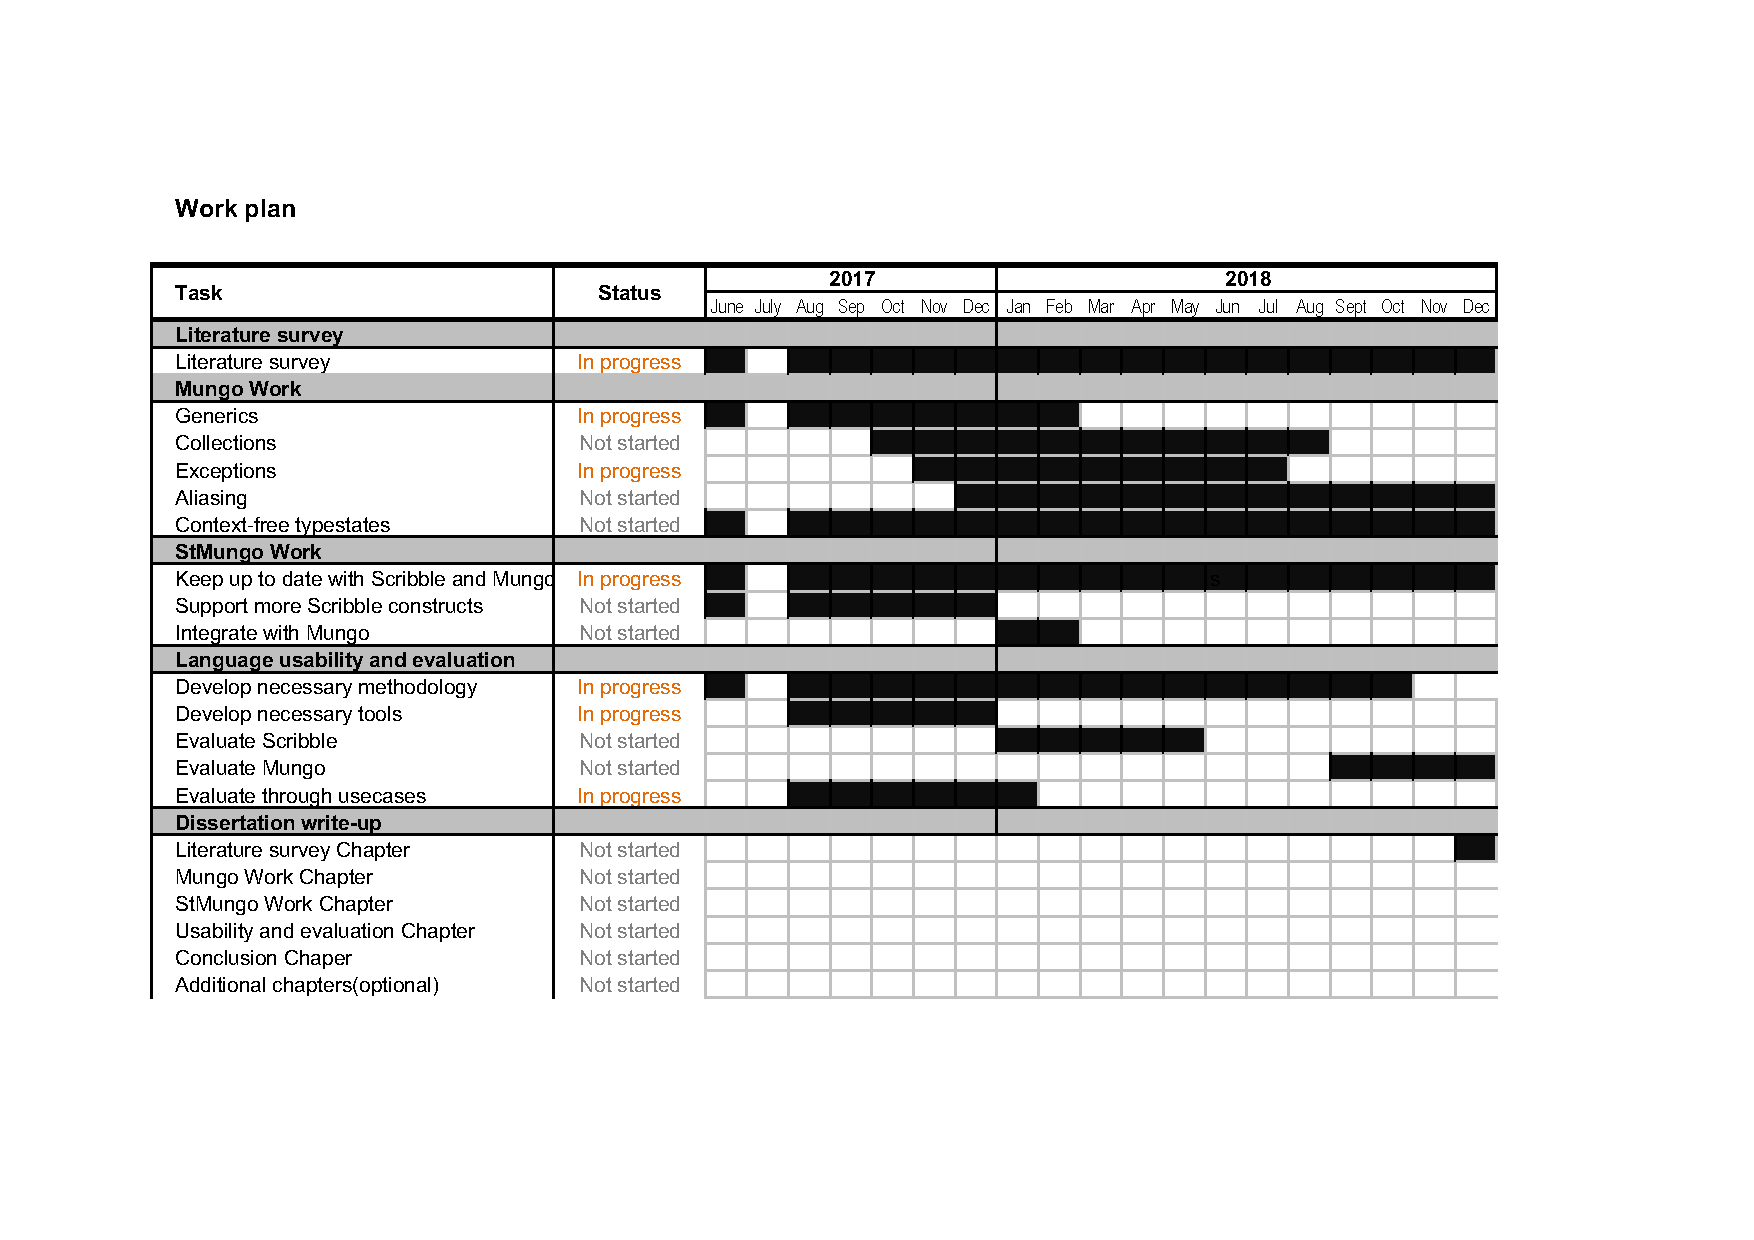
\includegraphics[height=0.9\vsize, width=1.1\hsize]{workplan.pdf}

    \caption{Caption in landscape to a figure in landscape.}
   \label{fig:LandscapeFigure}
\end{sidewaysfigure}
